\section{Flag 13 - NSA Image}

\paragraph{928d819fc19405ae09921a2b71227bd9aba106f9d2d37ac412e9e5a750f1506d}
\begin{center}
    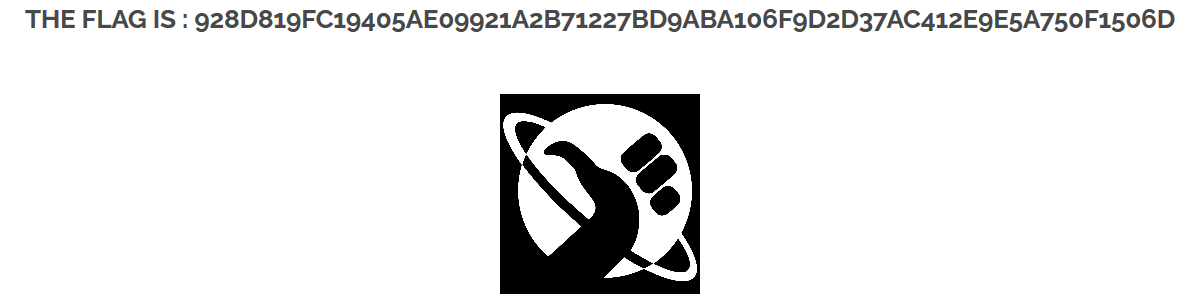
\includegraphics[width=0.5\textwidth]{16.Flag13/02-07.png}\\[0cm] 
\end{center}

\subsection{Vulnerability}

This attack is a form of XSS. XSS attacks enable attackers to inject client-side scripts into web pages viewed by other users. A cross-site scripting vulnerability may be used by attackers to bypass access controls such as the same-origin policy. The hijack of cookies and sessions is also common when conducting these kinds of attacks.

\subsection{Location}

'http://<ip-address>:80/index.php?page=media\&src=nsa'

\subsection{Method}

I opened the image and was redirected to the media page. I then noticed that the image was pointed to with a variable i.e 'src=nsa' in the URL `http://<ip-address>:80/index.php?page=media\&src=nsa`.

This is an immediate alert that MIME (Multipurpose Internet Mail Extension) might be valid.
The next step was to encode my own script on \href{https://hashes.com/en/tools/base64encode}{hashes.com} to encode my own script:

`<script>alert('sinkosi@itagain');</script>`

this returned the base64 string:

`PHNjcmlwdD5hbGVydCgnc2lua29zaUBpdGFnYWluJyk7PC9zY3JpcHQ+`

The next step was to make it run in the URL by changing src=nsa to the string:

`data:text/html;base64,PHNjcmlwdD5hbGVydCgnc2lua

29zaUBpdGFnYWluJyk7PC9zY3JpcHQ+`

The full URL is:

`http://<ip-address>:80/index.php?page=media\&src=data:text/html;

base64,PHNjcmlwdD5hbGVydCgnc2lua29zaUBpdGFnYWluJyk7PC9zY3JpcHQ+`

on reload of the page, the flag was retrieved


\subsection{Tools}

\begin{figure}[!htb]
    \centering
    \subfloat[Logo]{
\includegraphics[width=.45\columnwidth]{16.Flag13/02-01.png}\label{fig: 13-01 - wtf}} \quad
    \subfloat[Follow the logo]{
\includegraphics[width=.45\columnwidth]{16.Flag13/02-02.png}\label{fig: 13-02 - wrong}} \\
    \subfloat[Inspect code]{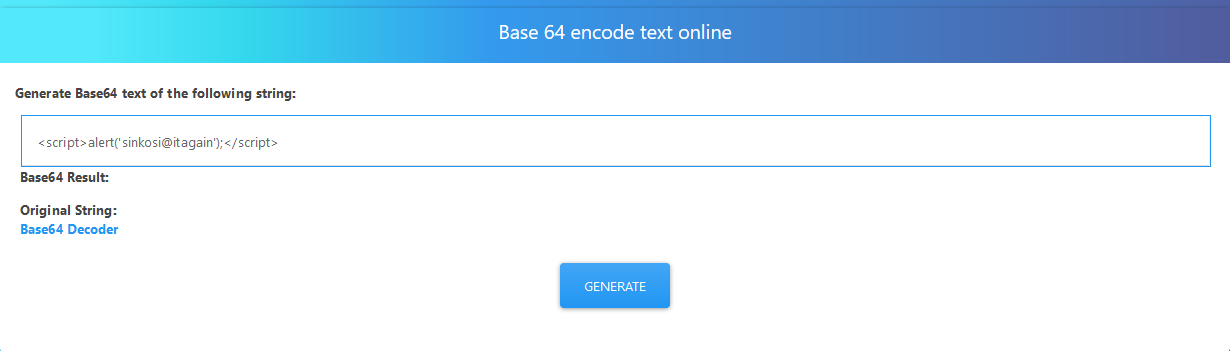
\includegraphics[width=.45\columnwidth]{16.Flag13/02-03.png}\label{fig: 13-03 - wtf}} \quad
    \subfloat[Base64 Decode]{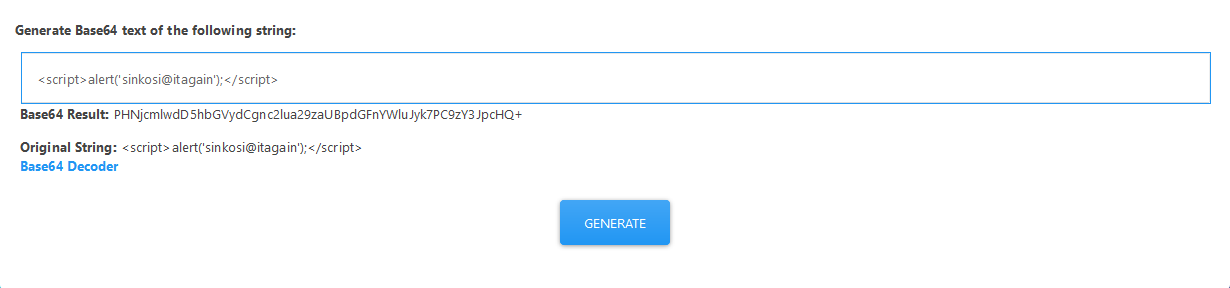
\includegraphics[width=.45\columnwidth]{16.Flag13/02-04.png}\label{fig: 13-04 - wrong}} \\
    \subfloat[Base64 Encode]{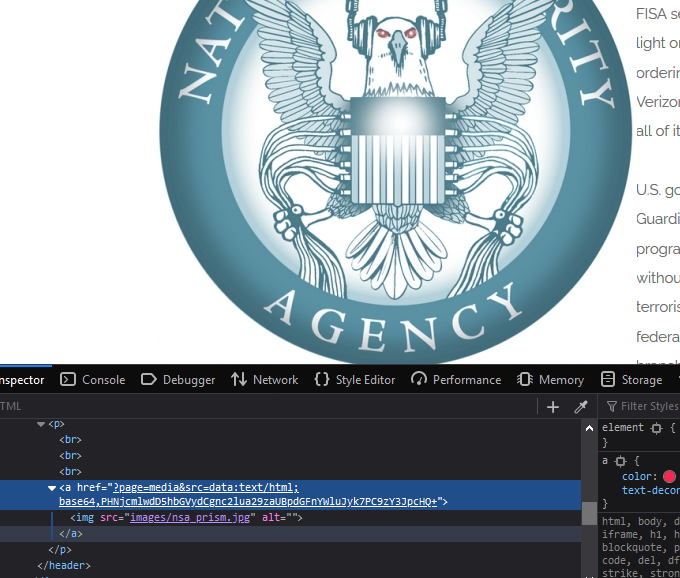
\includegraphics[width=.45\columnwidth]{16.Flag13/02-05.png}\label{fig: 13-05 - wtf}} \quad
    \subfloat[Reload new media]{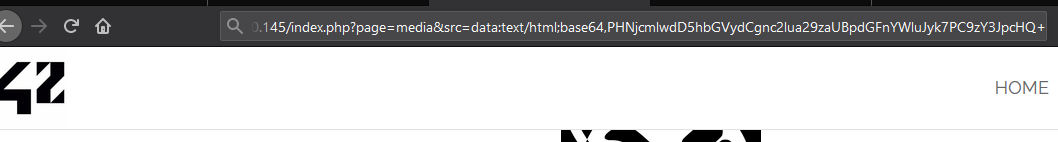
\includegraphics[width=.45\columnwidth]{16.Flag13/02-06.png}\label{fig: 13-06 - wrong}} \\
    \caption[Flag 13 Method]{Process to Capture the NSA XSS Flag} % The text in the square bracket is the caption for the list of figures while the text in the curly brackets is the figure caption
    \label{fig:flag13 method}
\end{figure}

\begin{itemize}
    \item \href{https://hashes.com/en/tools/base64encode}{hashes.com}
    \item \href{https://www.we45.com/blog/preventing-xss-with-base64-encoding-the-false-sense-of-web-application-security}{WE45}
    \item \href{https://github.com/OWASP/CheatSheetSeries/blob/master/cheatsheets/Cross_Site_Scripting_Prevention_Cheat_Sheet.md}{OWASP Cheatsheet}
\end{itemize}

\subsection{Remedy}

\begin{itemize}
    \item Sanitizing: Sanitizing user input is especially helpful on sites that allow HTML markup, to ensure data received can do no harm to users as well as your database by scrubbing the data clean of potentially harmful markup, changing unacceptable user input to an acceptable format.
    
    \item Input Validation: Validating input is the process of ensuring an application is rendering the correct data and preventing malicious data from doing harm to the site, database, and users.
    
    \item Escaping: Escaping data means taking the data an application has received and ensuring it’s secure before rendering it for the end user.
    
\end{itemize}